\documentclass[12pt]{article}
\usepackage{graphicx} % Required for inserting images
\usepackage{geometry}
\geometry{a4paper, margin=1in}
\usepackage{array}
\usepackage{emoji}
\usepackage{amsmath}
\usepackage{float} % for images


\begin{document}

\begin{center}
    \textbf{\Large IRVINE VALLEY COLLEGE} \\
    \vspace{0.2cm}
    \textbf{\Large PHYSICS LAB REPORT}
\end{center}

\vspace{1cm}

\begin{flushleft}
    \textbf{Course Number:} 62095 \\
    \textbf{Experiment Number:} 10 \\
    \textbf{Experiment Title:} Conservation of Angular Momentum \\
    \textbf{Date Performed:} November 4, 2024 \\
    \textbf{Due Date:} November 9, 2024
\end{flushleft}

\vspace{1cm}
\emoji{tulip}\emoji{tulip}\emoji{tulip}\emoji{tulip}\emoji{tulip}\emoji{tulip}\emoji{tulip}\emoji{tulip}\emoji{tulip}\emoji{tulip}\emoji{tulip}\emoji{tulip}\emoji{tulip}\emoji{tulip}\emoji{tulip}\emoji{tulip}\emoji{tulip}\emoji{tulip}\emoji{tulip}\emoji{tulip}\emoji{tulip}\emoji{tulip}\emoji{tulip}\emoji{tulip}\emoji{tulip}\emoji{tulip}\emoji{tulip}\emoji{tulip}
\begin{center}
    \begin{tabular}{|>{\centering\arraybackslash}m{5cm}|>{\centering\arraybackslash}m{5cm}|}
        \hline
        \textbf{RESEARCHER} & \textbf{SCALED GRADE} \\
        \hline
        Emma Truong & \underline{\hspace{2cm}} / 10 \\
        \hline
    \end{tabular}

    \vspace{1cm}

    \begin{tabular}{|>{\centering\arraybackslash}m{5cm}|>{\centering\arraybackslash}m{5cm}|}
        \hline
        \textbf{ANALYST} & \textbf{SCALED GRADE} \\
        \hline
        Roxanne Rahimi & \underline{\hspace{2cm}} / 10 \\
        \hline
    \end{tabular}

    \vspace{1cm}

    \begin{tabular}{|>{\centering\arraybackslash}m{5cm}|>{\centering\arraybackslash}m{5cm}|}
        \hline
        \textbf{PRINCIPLE INVESTIGATOR} & \textbf{SCALED GRADE} \\
        \hline
        Emma Truong / Roxanne Rahimi & \underline{\hspace{2cm}} / 10 \\
        \hline
    \end{tabular}
\end{center}


\section{Graphs}
\begin{figure}[H]
    \centering
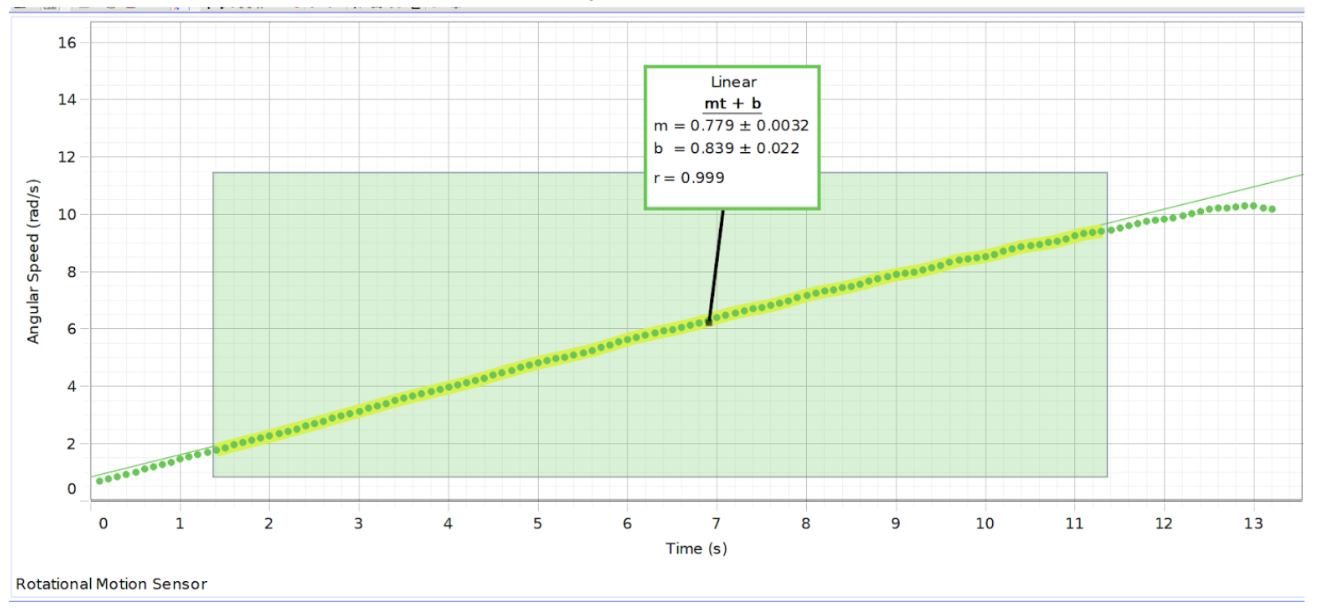
\includegraphics[width=0.75\linewidth]{Screw-Position-4.5.png}
    \caption{Screw Position at 4.5 cm}
    \label{fig:enter-label}
\end{figure}

\begin{figure}
    \centering
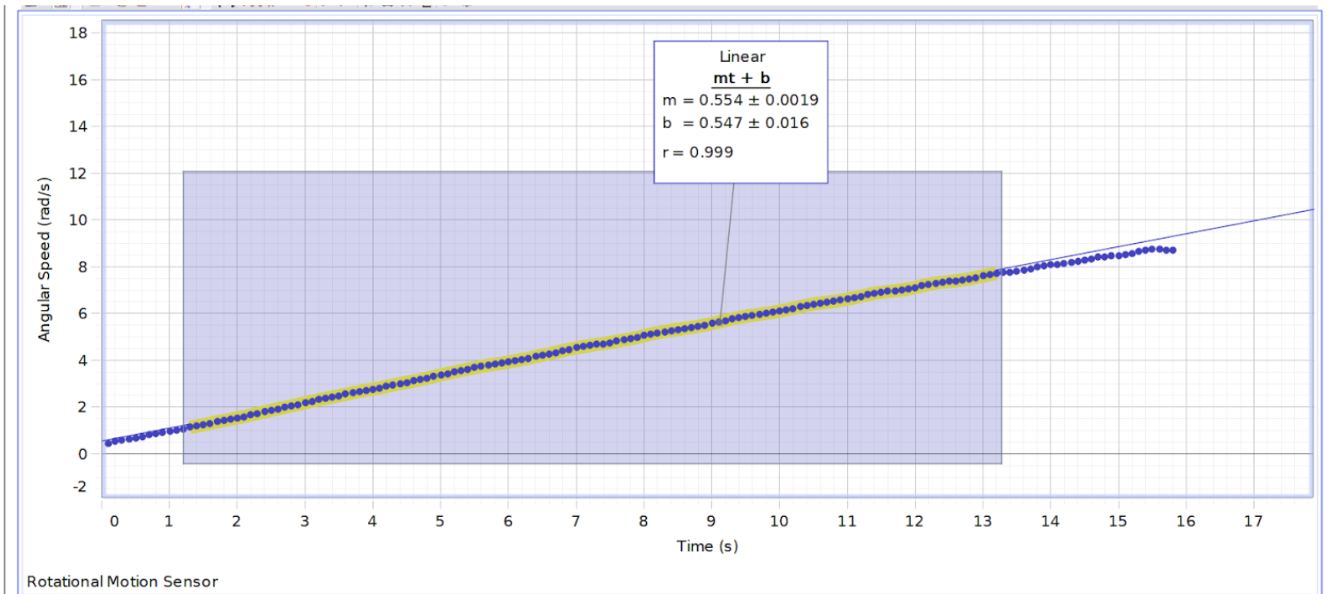
\includegraphics[width=0.75\linewidth]{screw-position 20.5 cm.png}
    \caption{Screw Position at 20.5 cm}
        \label{fig:enter-label}
\end{figure}

\begin{figure}
        \centering
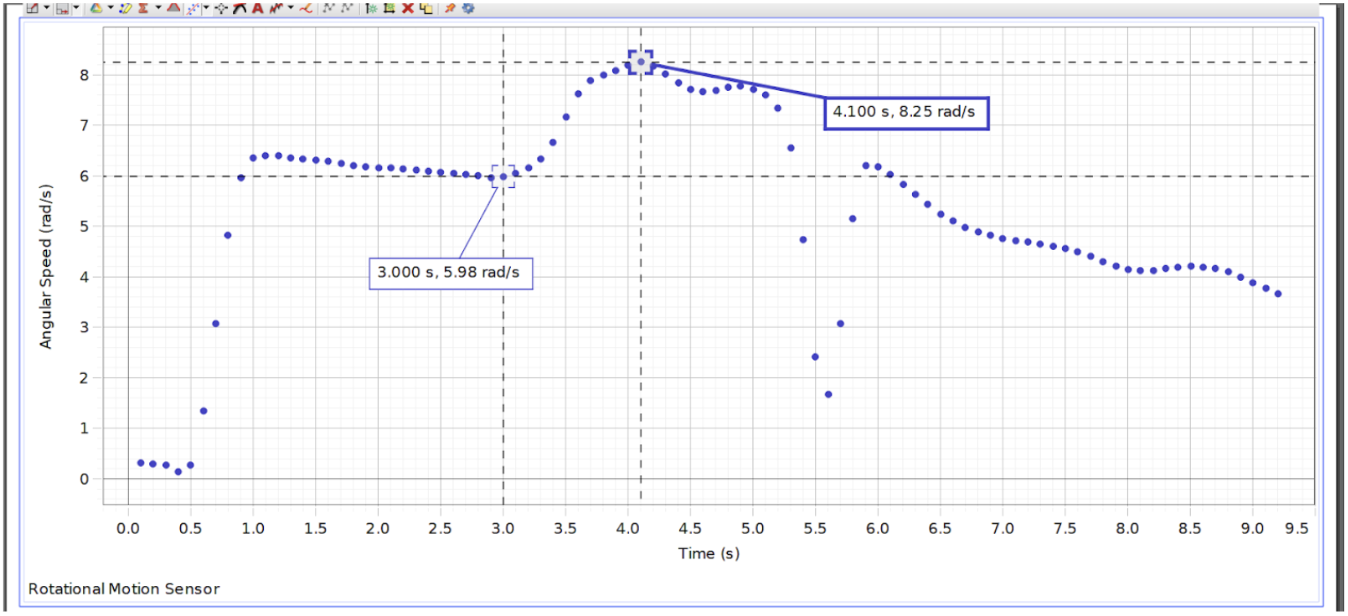
\includegraphics[width=0.75\linewidth]{Angular Speed.png}
        \caption{Angular Speed}
        \label{fig:enter-label}
    \end{figure}
\begin{figure}
    \centering
    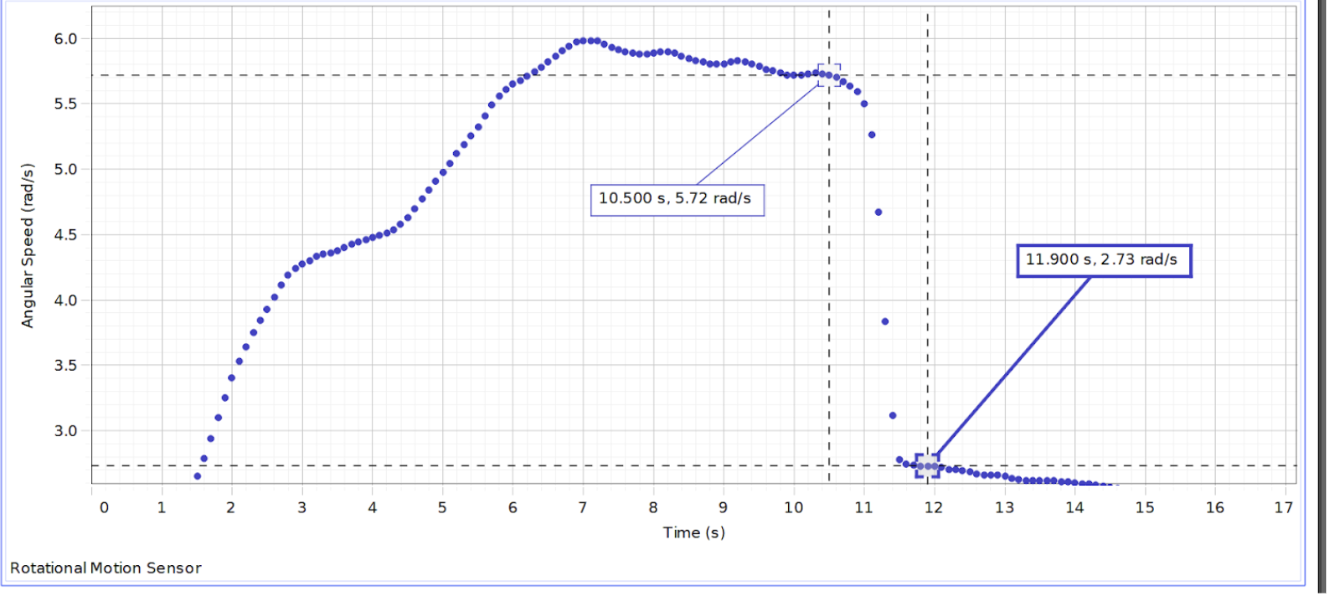
\includegraphics[width=0.75\linewidth]{Plastic Disk and Metal Ring.png}
    \caption{Plastic Ring and Metal Ring}
    \label{fig:enter-label}
\end{figure}

\section{Data Tables}

\vspace{1cm}

\begin{center}
    \textbf{DATA TABLE -- ROTATING PLATFORM}
\end{center}

\begin{center}
    \begin{tabular}{|>{\centering\arraybackslash}m{5cm}|>{\centering\arraybackslash}m{5cm}|}
        \hline
        \textbf{SPINDLE DIAMETER} & \textbf{7.35 ± 0.002} \\[0.2cm]
        \( d \pm \delta d \) (cm) & \\
        \hline
        \textbf{HANGING MASS' MASS} & \textbf{100.0 ± 0.1} \\[0.2cm]
        \( m \pm \delta m \) (g) & \\
        \hline
    \end{tabular}
\end{center}

\vspace{1cm}

\begin{center}
    \textbf{DATA TABLE -- POINT MASS}
\end{center}

\begin{center}
    \begin{tabular}{|>{\centering\arraybackslash}m{3cm}|>{\centering\arraybackslash}m{6cm}|>{\centering\arraybackslash}m{4cm}|}
        \hline
        \textbf{SCREW POSITION} & \textbf{ANGULAR ACCELERATION MAGNITUDE} & \textbf{ANGULAR SPEED} \\[0.2cm]
        & \( \alpha \pm \delta \alpha \) \(\left(\frac{\text{rad}}{\text{s}^2}\right)\) & \( \omega \pm \delta \omega \) \(\left(\frac{\text{rad}}{\text{s}}\right)\) \\
        \hline
        20.5 cm & 0.554 ± 0.0019 & 5.98 ± 0.01 \\
        \hline
        4.5 cm & 0.779 ± 0.0032 & 8.25 ± 0.01 \\
        \hline
    \end{tabular}
\end{center}

\vspace{1cm}

\begin{center}
    \textbf{DATA TABLE -- PLASTIC DISK AND METAL RING}
\end{center}

\begin{center}
    \begin{tabular}{|>{\centering\arraybackslash}m{5cm}|>{\centering\arraybackslash}m{5cm}|}
        \hline
        \textbf{ROTATING SYSTEM} & \textbf{ANGULAR SPEED} \\[0.2cm]
        & \( \omega \pm \delta \omega \) \(\left(\frac{\text{rad}}{\text{s}}\right)\) \\
        \hline
        Disk Only & 5.72 ± 0.01 \\
        \hline
        Disk \& Ring & 2.73 ± 0.01 \\
        \hline
    \end{tabular}
\end{center}
\section{Calculations}
\subsection{Square Mass at the 20.5 cm position}
\subsubsection{Initial Angular Momentum Magnitude}
$L_i = I\omega$
\newline
$L_i = \frac{1}{4}md^{2}\left(\frac{2g}{\alpha d} - 1\right)\omega$
\newline 
$L_i =\frac{1}{4}(0.1 \text{kg})(0.0735 \text{m})^{2}\left(\frac{2(9.8)}{(0.554)(0.0735) d} - 1\right)(5.98 \text{rad/s})$
\newline
$L_i = 0.39 \, \text{kg} \cdot \text{m}^2/\text{s}$
\subsubsection{Initial Angular Momentum Uncertainty}
$\delta L_i = \sqrt
{
\left(\frac
{\partial L_i}{\partial m}\right)^2(\partial m)^2+ 
\left(\frac
{\partial L_i}{\partial d}\right)^2(\partial d)^2+
\left(\frac
{\partial L_i}{\partial \omega}\right)^2(\partial \omega)^2+ \left(\frac
{\partial L_i}{\partial \omega}\right)^2(\partial \alpha)^2}$ 
\newline
\begin{equation}
\delta L_i = \sqrt{
    \begin{aligned}
        &\left( (\frac{1}{4}d^2)(\frac{2g}{\alpha d} - 1)\omega\right)^2(\delta m)^2 + \left( m\omega (\frac{g}{2\alpha}-\frac{d}{2})\right)^2(\delta d)^2 + \left( \frac{1}{4}md^2 (-\frac {2g}{\alpha ^2 d}-1)\omega\right)^2(\delta \alpha)^2 \\ &+ \left( \frac{1}{4}md^2(\frac{2g}{\alpha d}-1)\right)^2(\delta \omega)^2
    \end{aligned}
}
\end{equation}

\begin{equation}
\delta L_i = \sqrt{
    \begin{aligned}
        &\left( (\frac{1}{4}(0.0735)^2)(\frac{2(9.8)}{(0.554)(0.0735)} - 1)(5.98)\right)^2(0.0001)^2 + \left( (0.1)(5.98)(\frac{9.8}{2(0.554)})-\frac{0.0735} {2})\right)^2 \\ & (0.00002)^2 + \left( \frac{1}{4}(0.1)(0.0735)^2 (-\frac {2(9.8)}{(0.554)^2 (0.0735)}-1)(5.98)\right)^2(0.0019)^2 \\ &+ \left( \frac{1}{4}(0.1)(0.0735)^2(\frac{2(9.8)}{(0.554)(0.0735)}-1)\right)^2(0.01)^2
    \end{aligned}
}
\end{equation}
$\delta L_i = 8.7 \cdot 10^{-4} \, \text{kg} \cdot \text{m}^2/\text{s}$
\subsection{Square Mass at the 4.5 cm Position}
\subsubsection{Final Angular Momentum Magnitude}
$L_f = I\omega$
\newline
$L_f = \frac{1}{4}md^2(\frac{2g}{\alpha d}-1)\omega$
\newline
$L_f = \frac{1}{4}(0.1 \, \text{kg})(0.0735 \, \text{m})^2\left(\frac{2(9.8)}{(0.779)(0.0735)} -1 \right)(8.25)$
\newline
$L_f = 0.38 \, \text{kg} \cdot \text{m}^2 / \text{s}$
\subsubsection{Final Angular Momentum Magnitude Uncertainty}
$\delta L_i = \sqrt
{
\left(\frac
{\partial L_i}{\partial m}\right)^2(\partial m)^2+ 
\left(\frac
{\partial L_i}{\partial d}\right)^2(\partial d)^2+
\left(\frac
{\partial L_i}{\partial \omega}\right)^2(\partial \omega)^2+ \left(\frac
{\partial L_i}{\partial \omega}\right)^2(\partial \alpha)^2}$ 
\newline
\begin{equation}
\delta L_i = \sqrt{
    \begin{aligned}
        &\left( (\frac{1}{4}d^2)(\frac{2g}{\alpha d} - 1)\omega\right)^2(\delta m)^2 + \left( m\omega (\frac{g}{2\alpha}-\frac{d}{2})\right)^2(\delta d)^2 + \left( \frac{1}{4}md^2 (-\frac {2g}{\alpha ^2 d}-1)\omega\right)^2(\delta \alpha)^2 \\ &+ \left( \frac{1}{4}md^2(\frac{2g}{\alpha d}-1)\right)^2(\delta \omega)^2
    \end{aligned}
}
\end{equation}
\newline
\begin{equation}
\delta L_i = \sqrt{
    \begin{aligned}
        &\left( \frac{1}{4}(0.0735)^2(\frac{2(9.8)}{(0.779)(0.0735)} - 1)(8.25)\right)^2(0.0001)^2 + \left( (0.1)(8.25)(\frac{9.8}{2(0.779))}-\frac{(0.0735)}{2})\right)^2 \\ &(0.00002)^2 + \left( \frac{1}{4}(0.1)(0.0735)^2 (-\frac {2(9.8)}{(0.779) ^2 (0.0735)}-1)(8.25)\right)^2(0.0032)^2 \\ &+ \left( \frac{1}{4}(0.1)(0.0735)^2(\frac{2(Ω)}{(0.779)(0.0735)}-1)\right)^2(0.01)^2
    \end{aligned}
}
\end{equation}
$L_f = 0.001 \, \text{kg} \cdot \text{m}^2 / \text{s}$
\subsubsection{Angular Momentum Magnitude Percent Difference}
$PD = \left| \frac{0.39 - 0.38}{\frac{0.39+0.38}{2}}\right| \cdot 100\%$
\newline
$PD = 2.6\%$
\subsection{Ring and Disk}
\subsubsection{Disk Alone - using MOI calculation from previous lab}
$I_{disk} = 0.00937$
\newline
$L_i = I_{disk} \omega_{disk}$
\newline
$L_i = (0.00937)(5.72)$
\newline
$L_i = 0.0536 \, \text{kg} \cdot \text{m}^2 / \text{s}$
\subsubsection{Initial Angular momentum magnitude uncertainty}
$\delta L_i = \sqrt{(\omega_{disk})^2(\delta I_{disk})^2+(I_{disk})^2(\delta \omega_{disk})^2}$
\newline 
$\delta L_i = \sqrt{(5.72)^2(0.00031)^2+(0.00937)^2(0.01)^2}$
\newline
$\delta L_i = 0.00178 \, \text{kg} \cdot \text{m}^2 / \text{s}$
\subsubsection{Ring and Disk - using MOI  from previous lab}
$I_{disk + ring} = 0.01359 \, \text{kg} \cdot \text{m}^2$
\newline
$L_f =(I_{disk + ring})(\omega_{disk + ring})$
\newline
$L_f=(0.01359)(2.73)$
\newline
$L_f = 0.0371 \, \text{kg} \cdot \text{m}^2 / \text{s}$
\subsubsection{Final Angular Momentum Magnitude Uncertainty}
$\delta L_f = \sqrt{(\omega_{disk + ring})^2(\delta I_{disk + ring})^2+(I_{disk + ring})^2(\delta \omega_{disk + ring})^2}$
\newline 
$\delta L_f = \sqrt{(2.73)^2(0.00042)^2+(0.01359)^2(0.01)^2}$
\newline 
$L_f = 0.00115 \, \text{kg} \cdot \text{m}^2 / \text{s}$
\subsubsection{Percent Difference}
$PD = \left| \frac{(0.0536)-(0.0371)}{\frac{0.0536+0.0371}{2}}\right| \cdot 100 \%$
\newline 
$PD=36.38\%$
\section{table of values}
\begin{center}
    \textbf{TABLE OF RESULTS -- POINT MASS}
\end{center}

\begin{center}
    \begin{tabular}{|>{\centering\arraybackslash}m{4cm}|>{\centering\arraybackslash}m{4cm}|>{\centering\arraybackslash}m{4cm}|}
        \hline
        & \textbf{SCREW POSITION} & \\[0.2cm]
        & \textbf{20.5 cm} & \textbf{4.5 cm} \\
        \hline
        \textbf{MOMENT OF INERTIA} & 0.065 ± 0.000766 & 0.046 ± 0.000126
 \\[0.2cm]
        \( I \pm \Delta I \, \left( \text{kg m}^2 \right) \) & & \\
        \hline
        \textbf{ANGULAR MOMENTUM} & 0.39 ± $8.7 \cdot 10^{-4}$ & 0.38 ± 0.001 \\[0.2cm]
        \( L \pm \Delta L \, \left( \text{kg m}^2/\text{s} \right) \) & & \\
        \hline
        \textbf{PERCENT DIFFERENCE} & $2.6 \%$ & \\[0.2cm]
        \( PD \, \left( \% \right) \) & & \\
        \hline
    \end{tabular}
\end{center}

\vspace{1cm}

\begin{center}
    \textbf{TABLE OF RESULTS -- PLASTIC DISK AND METAL RING}
\end{center}

\begin{center}
    \begin{tabular}{|>{\centering\arraybackslash}m{4cm}|>{\centering\arraybackslash}m{4cm}|>{\centering\arraybackslash}m{4cm}|}
        \hline
        & \textbf{ROTATING SYSTEM} & \\[0.2cm]
        & \textbf{Disk Only} & \textbf{Ring \& Disk} \\
        \hline
        \textbf{ANGULAR MOMENTUM} & 0.0536 \pm 0.001738 & 0.0371 ± 0.00115 \\[0.2cm]
        \( L \pm \delta L \, \left( \text{kg m}^2/\text{s} \right) \) & & \\
        \hline
        \textbf{PERCENT DIFFERENCE} & 36.38 \% & \\[0.2cm]
        \( PD \, \left( \% \right) \) & & \\
        \hline
    \end{tabular}
\end{center}
\section{Questions}
\subsection{Overall, were your initial angular momentum magnitudes precise or imprecise? Justify your answer.}

Overall, our initial angular momentum magnitudes were very precise. We calculated and analyzed the uncertainty value for initial angular momentum (when the block was at 20.5 cm) which was 0.00087. This is a very small number showing that the initial angular momentum calculated from the experiment is close to the true value and thus very precise.

\subsection{Overall, were your final angular momentum magnitudes precise or imprecise? Justify your answer.}

Overall, our final angular momentum magnitudes were very precise. Our group determined this by calculating the uncertainty value for final angular momentum (when the block was at 4.5 cm) and we determined it to be 0.001. Upon analysis of this very small number, it can be concluded that the final angular momentum we calculated from the experiment is very close to the true value, showing that it is precise.

\subsection{Overall, was angular momentum conserved? If yes, then justify your answer. If not, identify the source of an unaccounted-for torque acting on the system.}

The conservation of momentum states that final momentum will be equal to initial momentum. In our experiment, our initial momentum was 0.39 $\text{kg} \cdot \text{m}^2 / \text{s}$ while our final momentum was 0.38 $\text{kg} \cdot \text{m}^2 / \text{s}$ 
While these two values are indeed close, they are not equal to each other meaning momentum was overall not conserved.
A possible source of unaccounted for torque acting on the system could have been that the string on the spindle was placed on slightly differently offset positions between each trial. Or, the string could have also not been perfectly aligned on the spindle. 

\subsection{Identify the independent variable(s) for this experiment.
Be specific and use proper vocabulary.}

The independent variables for this experiment would be the screw position of the square mass at the 20.5 cm and 4.5 cm position. These two values were known before the procedure and were not influenced by the experiment. Rather, they served as factors that could be manipulated in order to obtain the results of the experiment. This shows that they are independent variables.

\subsection{Identify the fixed variable(s) for this experiment.
Be specific and use proper vocabulary.}

The fixed variables for this experiment are the spindle diameter (7.35 cm)  and the mass of the hanging mass (100g). These values were held constant throughout the entire experiment and were never changed or manipulated. These features of the experiment stayed the same in order for us to obtain consistent results, making them fixed variables.

\subsection{Identify the dependent variable(s) for this experiment.
Be specific and use proper vocabulary.}

The dependent variables for this experiment were the angular acceleration and the angular speed of the hanging mass as it descended to the ground. This is because these values were not known before the experiment, rather they needed to be recorded as a result of the experiment. The acceleration and speed were also manipulated and changed based on the the location of the square mass between the screws at 20.5 and 4.5 cm (the independent variables).  Because the result of these values were a result of the independent variables, the angular acceleration and angular speed are the dependent variables.

\subsection{Conclusion}
This experiment aimed to show the conservation of angular momentum and display how changes in the system in terms of mass for example affect the moment of inertia and therefore angular momentum. To dive into this, the results indicate a noticeable percent difference of 36.38\% between the calculated moment of inertia for the disk alone and the combined disk and ring. The large percent difference can be caused by the increased mass of the ring + disk system when compared to the mass of just the disk. A source of error could be small misalignment or shifts in the position of the ring relative to the disk which could lead to large differences in the measured rotational inertia, especiallywhen the mass is further from the center of rotation - as it is in the 20.5 cm situation. Also, friction at the pivot could cause some slight deviations in the true answer.
\end{document}

